\RequirePackage{luatex85}
\documentclass[tikz]{standalone}
% Default preamble
\usepackage{pgfplots}
\pgfplotsset{compat=newest}
\usepgfplotslibrary{groupplots}
\usepgfplotslibrary{polar}
\usepgfplotslibrary{smithchart}
\usepgfplotslibrary{statistics}
\usepgfplotslibrary{dateplot}
\usepgfplotslibrary{ternary}
% Custom preamble from global variable:
\usetikzlibrary{patterns}
\usepackage{xcolor}
\definecolor{cred}{HTML}{ED1C24}
\definecolor{cgrey}{HTML}{7F7F7F}
\definecolor{cblue}{HTML}{00A2E8}
\definecolor{cgreen}{HTML}{22B14C}
\definecolor{cyellow}{HTML}{FFF200}
\definecolor{corange}{HTML}{EA7904}
\definecolor{cpurple}{HTML}{9100FC}
\definecolor{julia1}{HTML}{1F77B4}
\definecolor{julia2}{HTML}{FF7F0E}
\definecolor{julia3}{HTML}{2CA02C}
\definecolor{julia4}{HTML}{D62728}
\begin{document}
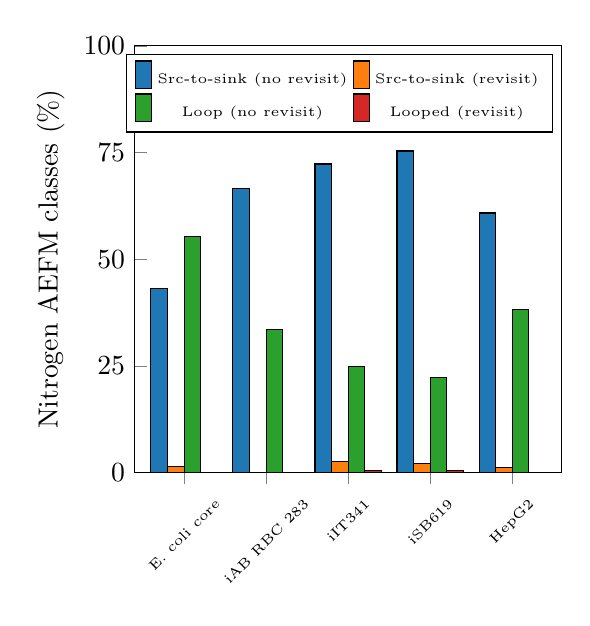
\begin{tikzpicture}
\begin{axis}[height={7cm}, width={7cm}, ybar = 0pt, xmajorgrids={false}, ymajorgrids={false}, xtick pos = bottom, ytick pos = left, bar width = 6pt, enlarge x limits = 0.15, enlarge y limits = false, legend image code/.code={\draw [#1] (0cm,-0.1cm) rectangle (0.2cm,0.25cm); }, legend style={legend columns={2}, font=\tiny}, ymax={100}, ymin={0}, xmax={5}, xtick={1,2,3,4,5}, xticklabels={E. coli core,iAB RBC 283,iIT341,iSB619,HepG2}, xticklabel style = {font=\tiny, align=center,rotate=45}, ytick={0,25,50,75,100}, ylabel={Nitrogen AEFM classes (\%)}]
    \addplot[black, fill=julia1]
        coordinates {
            (1,43.13725490196079)
            (2,66.47537063605931)
            (3,72.29885057471265)
            (4,75.3552835232869)
            (5,60.82272282076395)
        }
        ;
    \addplot[black, fill=julia2]
        coordinates {
            (1,1.4705882352941175)
            (2,0.0)
            (3,2.5766283524904217)
            (4,2.0472773322076825)
            (5,1.0773751224289911)
        }
        ;
    \addplot[black, fill=julia3]
        coordinates {
            (1,55.392156862745104)
            (2,33.5246293639407)
            (3,24.760536398467433)
            (4,22.21049669340087)
            (5,38.09990205680705)
        }
        ;
    \addplot[black, fill=julia4]
        coordinates {
            (1,0.0)
            (2,0.0)
            (3,0.36398467432950193)
            (4,0.38694245110454484)
            (5,0.0)
        }
        ;
    \legend{{Src-to-sink (no revisit)},{Src-to-sink (revisit)},{Loop (no revisit)},{Looped (revisit)}}
\end{axis}
\end{tikzpicture}
\end{document}
